\documentclass{article}
\usepackage[utf8]{inputenc}
\usepackage{graphicx}
\usepackage[
backend=biber,
style=authoryear,
citestyle=authoryear
]{biblatex}
\renewcommand*{\bibfont}{\small}
\usepackage[normalem]{ulem}
\usepackage{fancyhdr}
\usepackage{multicol}
\usepackage[hidelinks]{hyperref}
 
\pagestyle{fancy}
\fancyhf{}
\rhead{The Causal Effect of Media Frames}
\lhead{Nicolai Berk}
\cfoot{\thepage}

\useunder{\uline}{\ul}{}

\addbibresource{PhD-Proposal.bib}


\usepackage{xcolor}

\title{The Causal Effect of Media Frames on Issue Attitudes}
\author{Nicolai Berk\footnote{Doctoral Candidate, Dynamics Doctoral Program, Humboldt-Universität zu Berlin, \href{mailto:nicolai.berk@hu-berlin.de}{nicolai.berk@hu-berlin.de}}}
\date{September 2021}

\begin{document}

\maketitle


\begin{abstract}
    A large body of literature debates the existence and extent of effects of media framing on consumers' issue attitudes. Combining panel data from the German Longitudinal Election Study with a fine-grained analyses of media framing, I address this debate with observational data, providing evidence from 1,752 fixed-effect, difference-in-differences models suggesting systematic differences in newspaper readers' opinion shifts. Second, I show that such changes in consumers' attitudes towards immigration surrounding the German national election 2017 did \textit{not} correspond to changes in the migration framing of consumed media outlets. The findings contribute to our understanding of opinion formation processes and the relevance of the news media in the 21st century.
\end{abstract}


\section{Introduction}


How does news media content affect citizens' issue attitudes? Research on political behaviour has discussed this question for nearly a century. Classic theories of agenda setting hold that the attention devoted to issues in the news media will guide citizens to consider these issues important (\cite{McCombs1972}). Similarly, the literature on framing expects that the presentation of issues in the news media will affect recipients' opinions about these issues (\cite{Nelson1997}). Both theories suggest that media coverage strongly affects citizens' understanding of and opinions about politics.

Yet, a popular critique of these theories maintains that strong news effects are unlikely in the modern media environment, where consumers self-select into news sources of their liking. As a result, "most media users will rarely find themselves in the path of attitude-discrepant information". Even if consumers had to face such discrepant information, this should reinforce their existing views rather than persuade as they are used to a partisan media diet (\cite[724f]{Bennett2008}). Similarly, agenda setting effects are unlikely as a result of selective exposure (\cite{Lau2021}).

This conflicting evidence begs the question: when can we expect media framing effects? Some authors have argued that a lack of media effects can be explained by readers who discount a publications' bias. For example, when a left-wing newspaper endorses a left-wing candidate, this should have no effect on citizens' assessment of the candidate, as the endorsement was to be expected (\cite{Chiang2011a}, see also \cite{Spirig2020}). Additionally, citizens might take cues from their preferred publication because they developed trust in its coverage over time.

The present study contributes to this debate in two ways. First, instead of taking media slant as a given (\cite{Foos2020, Guess2021}), I measure the prevalence of different frames directly and assess whether their presence in the media across time affected readers' issue attitudes. Second, I use the variation in framing \textit{within} a given newspaper across time as the main independent variable. Many other studies explored effects of changes in newspaper consumption (\cite{Foos2020, Gentzkow2011}) or randomly assigned participants to consume certain news media rather than others (\cite{Guess2021}). However, readers usually do not change readership, nor are all newspapers equally credible to them. If trust in a given news source matters, or if readers' discount publications' bias, such designs are unlikely to measure how news consumption affects consumers' opinions. This paper hence assesses how the changing framing of a salient issue within an already consumed paper changes citizens' attitudes. 

\section{Framing in the wild}

\subsection{General evidence of framing effects}

A large amount of evidence underlines the importance of newspaper coverage for political opinion formation. Observational evidence shows that newspaper exposure (\cite{Foos2020, Spirig2020}), endorsements of specific candidates (\cite{Ladd2009a, Chiang2011a}), coverage of specific topics (\cite{King2017}), reports on political parties (\cite{Boomgaarden2009, Devine2020}), internet access (\cite{Schaub2020}), and changes in television news content (\cite{Durante2012}) have affected which issues citizens care about, their opinion about these issues, and their voting behaviour. An even larger body of experimental work reports strong effects of issue framing on participants' issue attitudes (see \cite{Busby2019} for a recent overview).

This "maximal effects" view is contrasted by a body of evidence indicating weak to absent media effects as well. \citeauthor{Gentzkow2011} show that even historically, the entry and exit of newspapers in the US does affect turnout, but that the newspapers' slant does not affect either party's vote share. They conclude that "the persuasive effect of partisan newspapers is limited" (\citeyear[3011]{Gentzkow2011}). Recently, \citeauthor{Guess2021} incentivised participants of an online-panel to visit left- or right-leaning news websites, with no effect on opinions (\citeyear{Guess2021}). An experiment by \citeauthor{Lau2021} indicates that increasing the likelihood of encountering information about a fictitious candidate's stance on a given issue does not increase the importance of that issue in reaching a voting decision, directly contradicting theories of agenda setting. This lack of evidence echos a general critique of the external validity of framing experiments and other experimental evidence about opinion formation (\cite{Barabas2010, Busby2019, Leeper2020}).

What might explain these different findings? Scope conditions for media effects seem to be surprisingly understudied given the contradicting body of evidence. \citeauthor{Chiang2011a} argue that endorsements from newspapers with ideological leanings neutral or opposite to the endorsed party/candidate should have stronger effects on voting behaviour, as voters discount the general bias of a newspaper (\citeyear{Chiang2011a}). \citeauthor{Spirig2020} shows that the takeover of a Swiss regional newspaper through a leading politician of the far-right and the subsequent change in its political slant had no effect on citizens' voting behaviour and suggests that this is a result of voters discounting the new owner's political slant and stopping to read the newspaper.

If citizens discount the content of newspapers, they should not react to news content which is randomly assigned to them. Instead, a most likely case for effects of news exposure would have to assess changing content \textit{within} the same newspapers and its effect on consumers' issue attitudes. This is precisely what this study aims to do.

\subsection{Agenda Setting}

\textbf{[Now that there seem to be no framing effects, I am considering to make this a broader study of media effects and include agenda setting. But I guess this might be hard to finish until the weekend, so I should probably drop it for now. Might still be relevant for future direction of the paper]}\medskip

[Insert discussion of McCombs \& Shaw, as well as recent studies on agenda setting through the media, might also contrast 'latent salience model' (similar to Gamson \& Modigliani) and 'direct agenda setting']

\medskip

\textbf{H1a (direct agenda setting):} The more an issue is emphasised in a given newspaper, the more important this issue is considered by readers of this newspaper, relative to other newspapers.

\textbf{H1b (latent salience model):} Increased issue attention in the news across time corresponds to increased importance among all readers, but higher attention in one newspaper compared to others does not increase the perceived importance among its readers relative to those of other newspapers (all move at the same time).

\subsection{Mechanisms of Framing}

While news slant is a very general concept, and sometimes operationalised as similarity to specific parties' communication (\cite{Gentzkow2010}) or issue positions/tonality (\cite{Spirig2020}), framing theory provides a specific expectation about which treatment should affect which issue attitudes how. As \citeauthor{Nelson1997} write: "framing is the process by which a communication source, such as a news organisation, defines and constructs a political issue or public controversy" (\citeyear[567]{Nelson1997}). A "frame" is then the operating unit of this process, defining the issue at hand in a specific way. Different forms of frames have been conceptualised. When I talk about 'frames' here, I refer to \textit{emphasis frames}. These frames emphasise certain topics in relation to an issue, guiding the recipient to think about the issue with those considerations in mind that are promoted by the frame (\cite[153f]{Leeper2020}). For example, issues of increasing welfare contributions might be discussed with reference to inequality and providing chances to the poor, or by mentioning that higher welfare benefits might result in higher taxes. Individuals' support of a statement will differ dependent on the frame presented (\cite{sniderman2004structure}).

While this broad definition gives a first idea of what framing is about, the concept of emphasis framing has been criticised for being too broad and imprecise to contribute anything meaningful to the field (\cite{Scheufele2012}). To address this shortcoming, I follow the framing literature building on the \textit{value-expectancy model} (\cite{Ajzen2000, Nelson1997}). This model suggests that an attitude on a given issue is a function of two things: considerations and their respective weights. The evaluation of the issue is subdivided into a number of considerations (to which political scientists might refer as "valence issues"), that will be easier to evaluate. For example, to decide whether a lockdown is necessary to battle the spread of Covid-19 in one's country, a person might consider the detrimental short-term effect on businesses and individuals' mental health (negative considerations), as well as the cost of overburdened hospitals and additional deaths (positive considerations, at least with respect to the evaluation of a lockdown). Individuals weigh each of these considerations to form an overall opinion on the subject. 

Figure \ref{fig:cogStor} visualises this logic. A given issue is associated with an attitude or evaluation $y$. The issue is related to a number of different considerations, each of which carries an associated evaluation $x_i$, e.g. that the prevention of overcrowded hospitals is a good thing. Each of these considerations is more or less associated with the issue. Based on the strength of this association $w_i$, a given consideration's evaluation is more or less reflected in the issue evaluation $y$, which is equal to the weighted sum of considerations. Emphasis framing affects the issue attitude $y$ by changing the weights of different considerations\footnote{Note that this concept of framing is identical to second-level or attribute agenda setting (\cite{Lopezescobar2017, McCombs2000}; see \cite[174]{Mclaren2018} for a discussion of the overlap of these literatures). I will stick to the framing perspective here as the literature is focused on issues rather than candidates' attributes, and the conceptualisation as frame allows to form expectations about citizens' reactions to changing news frames.}.

This operationalisation allows us to generate specific expectations about how frames in the news media affect respondents' issue opinions. When presented with an emphasis frame on a given issue, the respondents' cognitive association of the issue with the emphasised consideration should increase, thus changing the evaluation of the issue by increasing the importance of the consideration. If the consideration is positive (towards the issue), the attitude towards the issue should improve, and the opposite when it is negative. \medskip

\textbf{H2 (emphasis framing):} If a newspaper emphasises more positive/negative frames of an issue, the readers' attitude about the issue should become more positive/negative.

% JB: I’m wondering if negative reference might help you with the definition. In our last colloquium you still got the criticism that framing was not well defined enough. I think you might be able to avoid a lot of the criticism (what makes framing different from issue ownership etc.) by addressing the contrast from framing from some of the more used concepts such as issue attention. Just an idea
% \footnote{I will stop here to outline the other chapters. However, a future version of this draft will discuss the cognitive basis of this model (considerations: affective storage as discussed by Taber and Lodge, Kunda; weights: physical cognitive association through Hebbian learning) and  whether this is a rational model (\cite{Ajzen2000, Druckman2001}).}.

\begin{center}
\begin{figure}
    \centering
    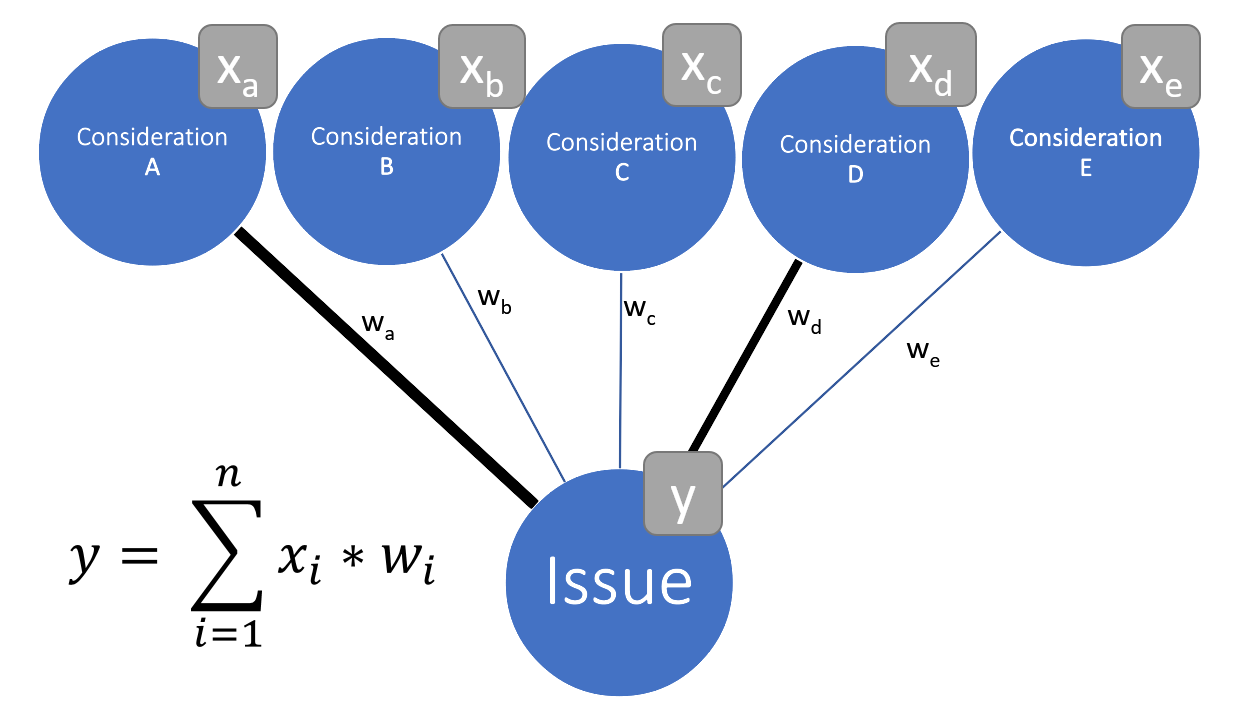
\includegraphics[width=\textwidth]{pres/vis/CognitiveStorage.png}
    \caption{The cognitive evaluation of an issue $y$ is determined by the strength of association $w_i$ with other concepts with existing evaluations $x_i$.}
    \label{fig:cogStor}
\end{figure}
\end{center}



\section{Study design}

\subsection{Case description}


[describe context of German election 2017 and dominance of migration topic]

\subsection{Public opinion data}

To measure the dependent variable (issue attitudes) and differentiate the treatment groups (newspaper readers), I employ panel data from the German Longitudinal Election Study (GLES, \cite{GLES2019LongTermTracking}). The panel consists of 15 waves, of which 6 (4) contain variables on newspaper consumption and immigration (integration) attitudes. In each wave 9,000-15,000 respondents were interviewed, which allows the precise estimation of effects of media consumption.

Figure \ref{fig:issues} shows the two main dependent variables for each group of readers. Note that higher values on the immigration variable indicate more restrictive attitudes, while higher values on the integration variable are most liberal. As can be seen, readers of the tabloid 'Bild' differ strongly from consumers of other outlets, with far more restrictive attitudes. Both variables seem inversely correlated (as expected), with values moving towards the more liberal pole until autumn, where the trend is reversed. The development of issue importance across time can be found in Appendix \ref{app:importance}.

\begin{figure}[!ht]
    \centering
    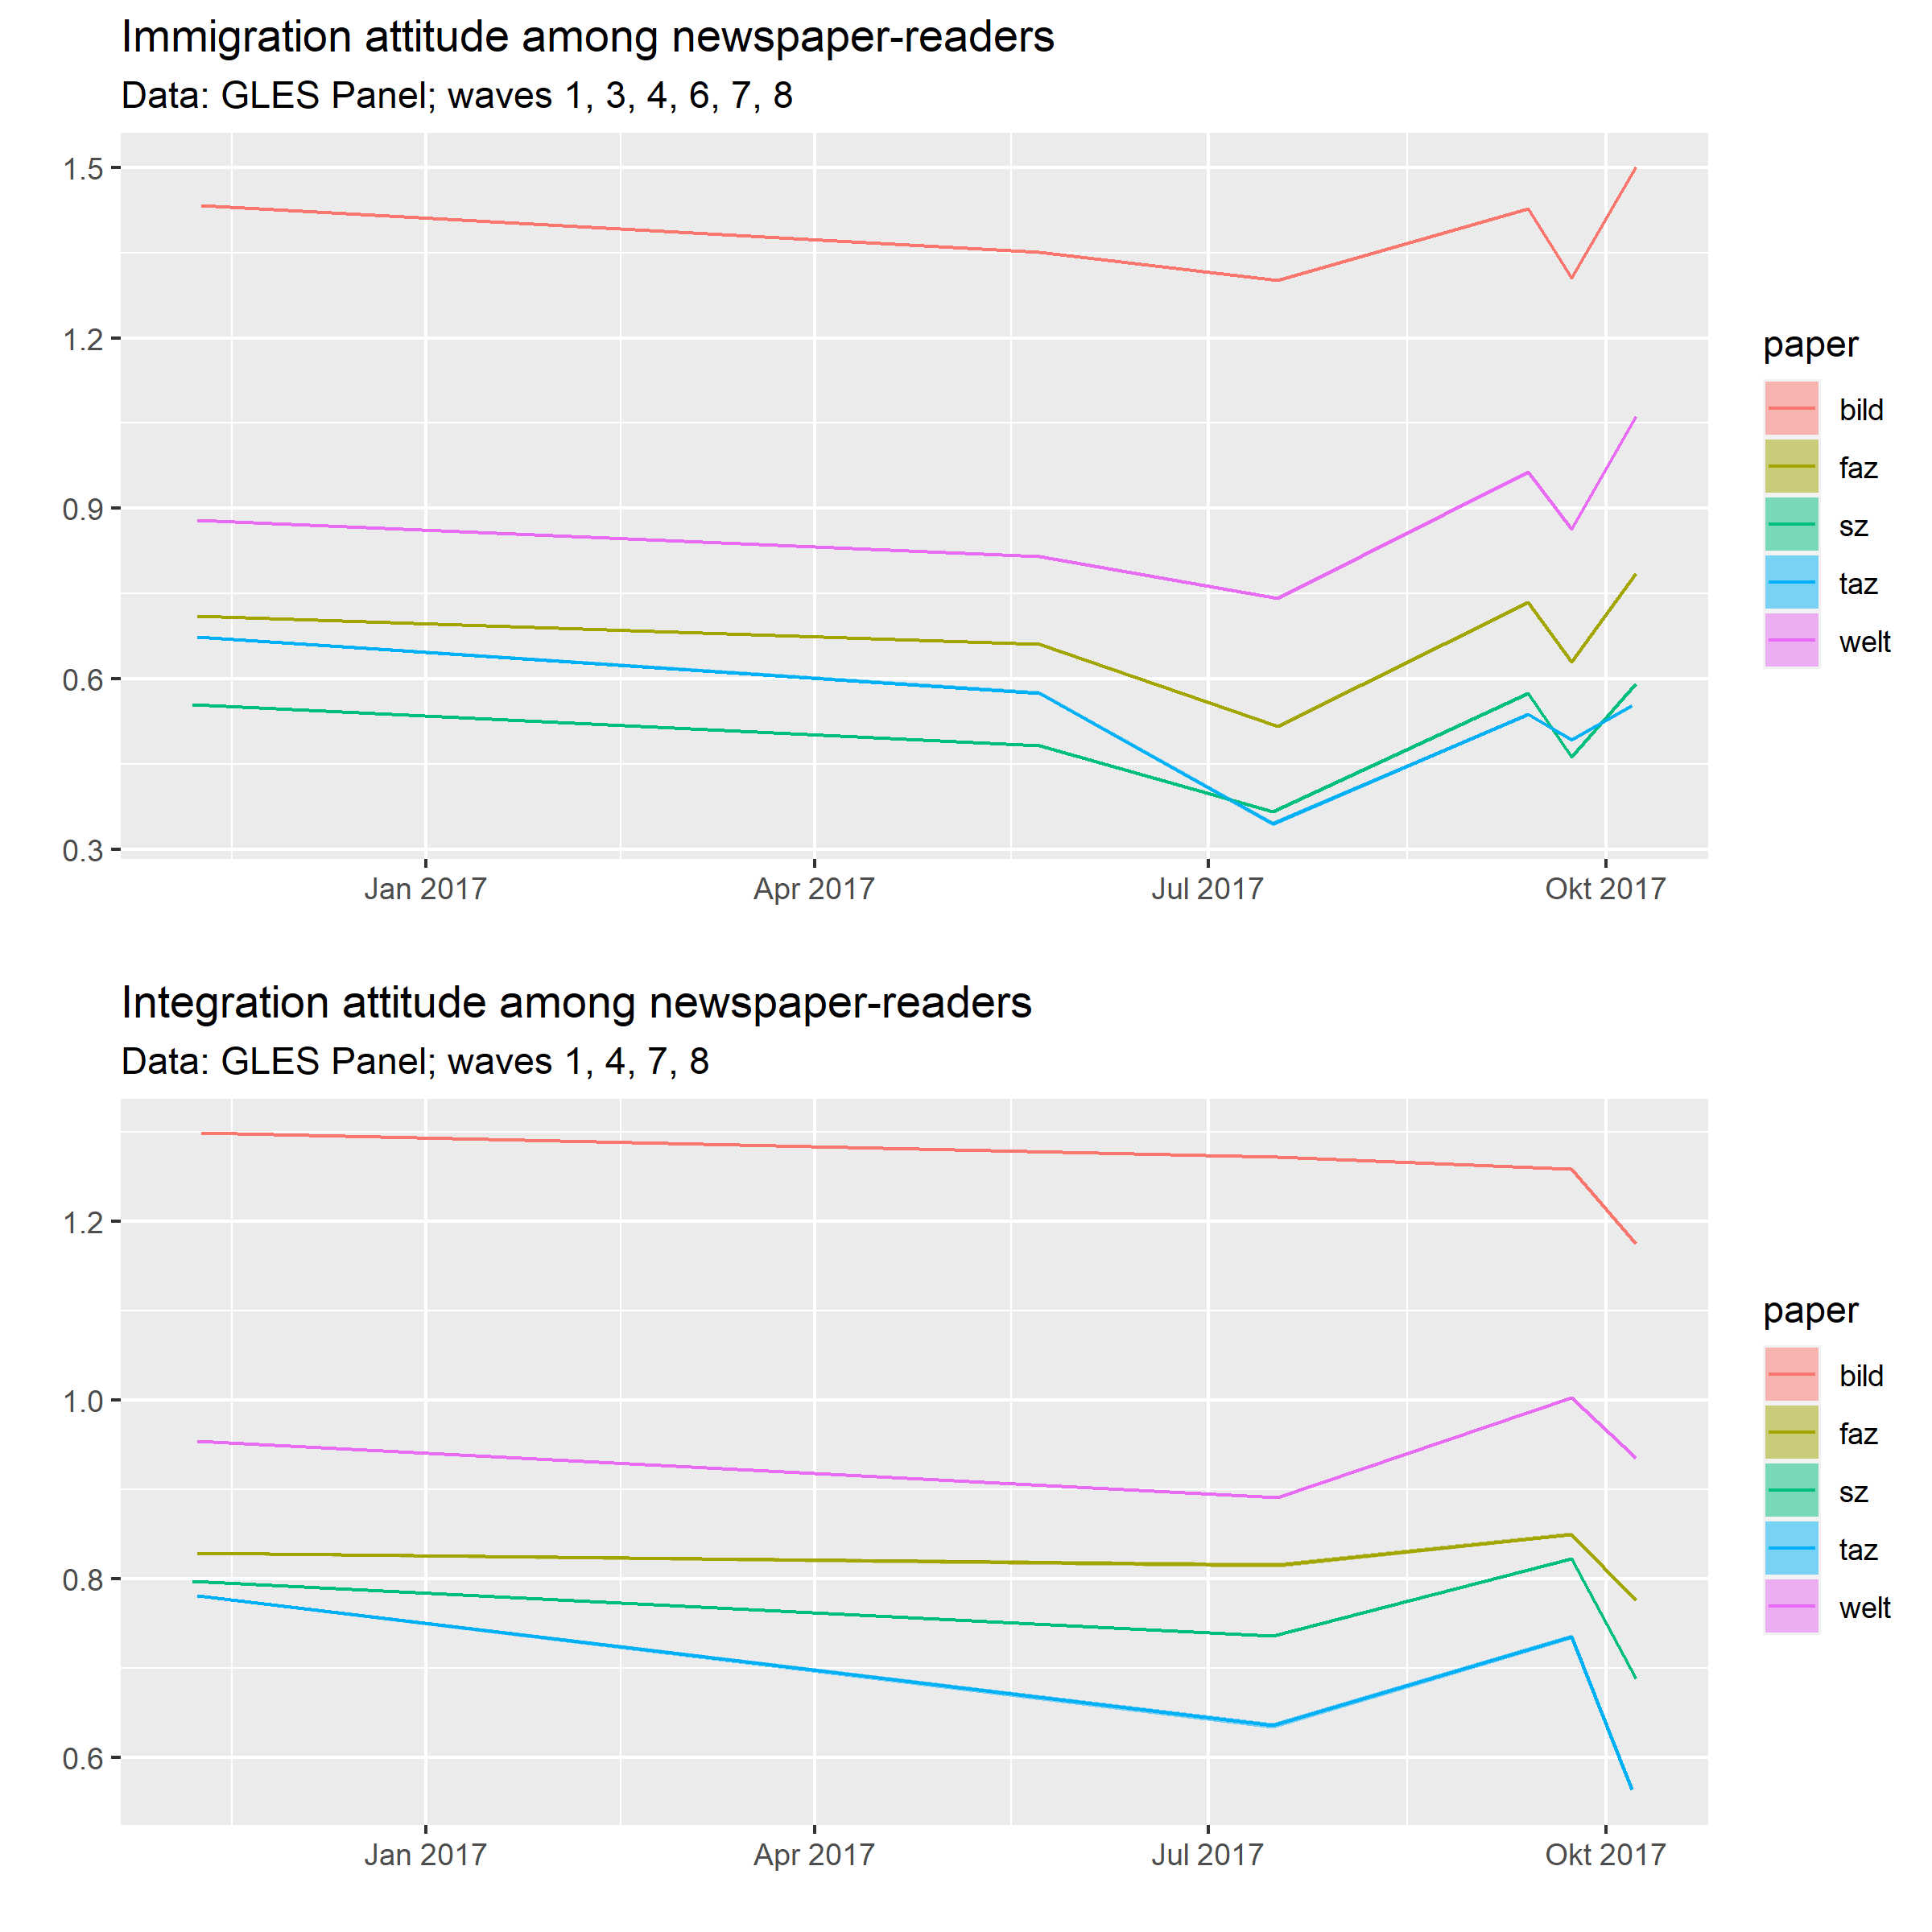
\includegraphics[width=\textwidth]{paper/vis/issues_readers.png}
    \caption{Opinions on migration and integration across time (higher values on immigration indicate more restrictive attitudes, vice versa for integration).}
    \label{fig:issues}
\end{figure}


\subsection{Measuring news framing}

\subsubsection{Measuring news attention to migration}



\begin{figure}[!ht]
    \centering
    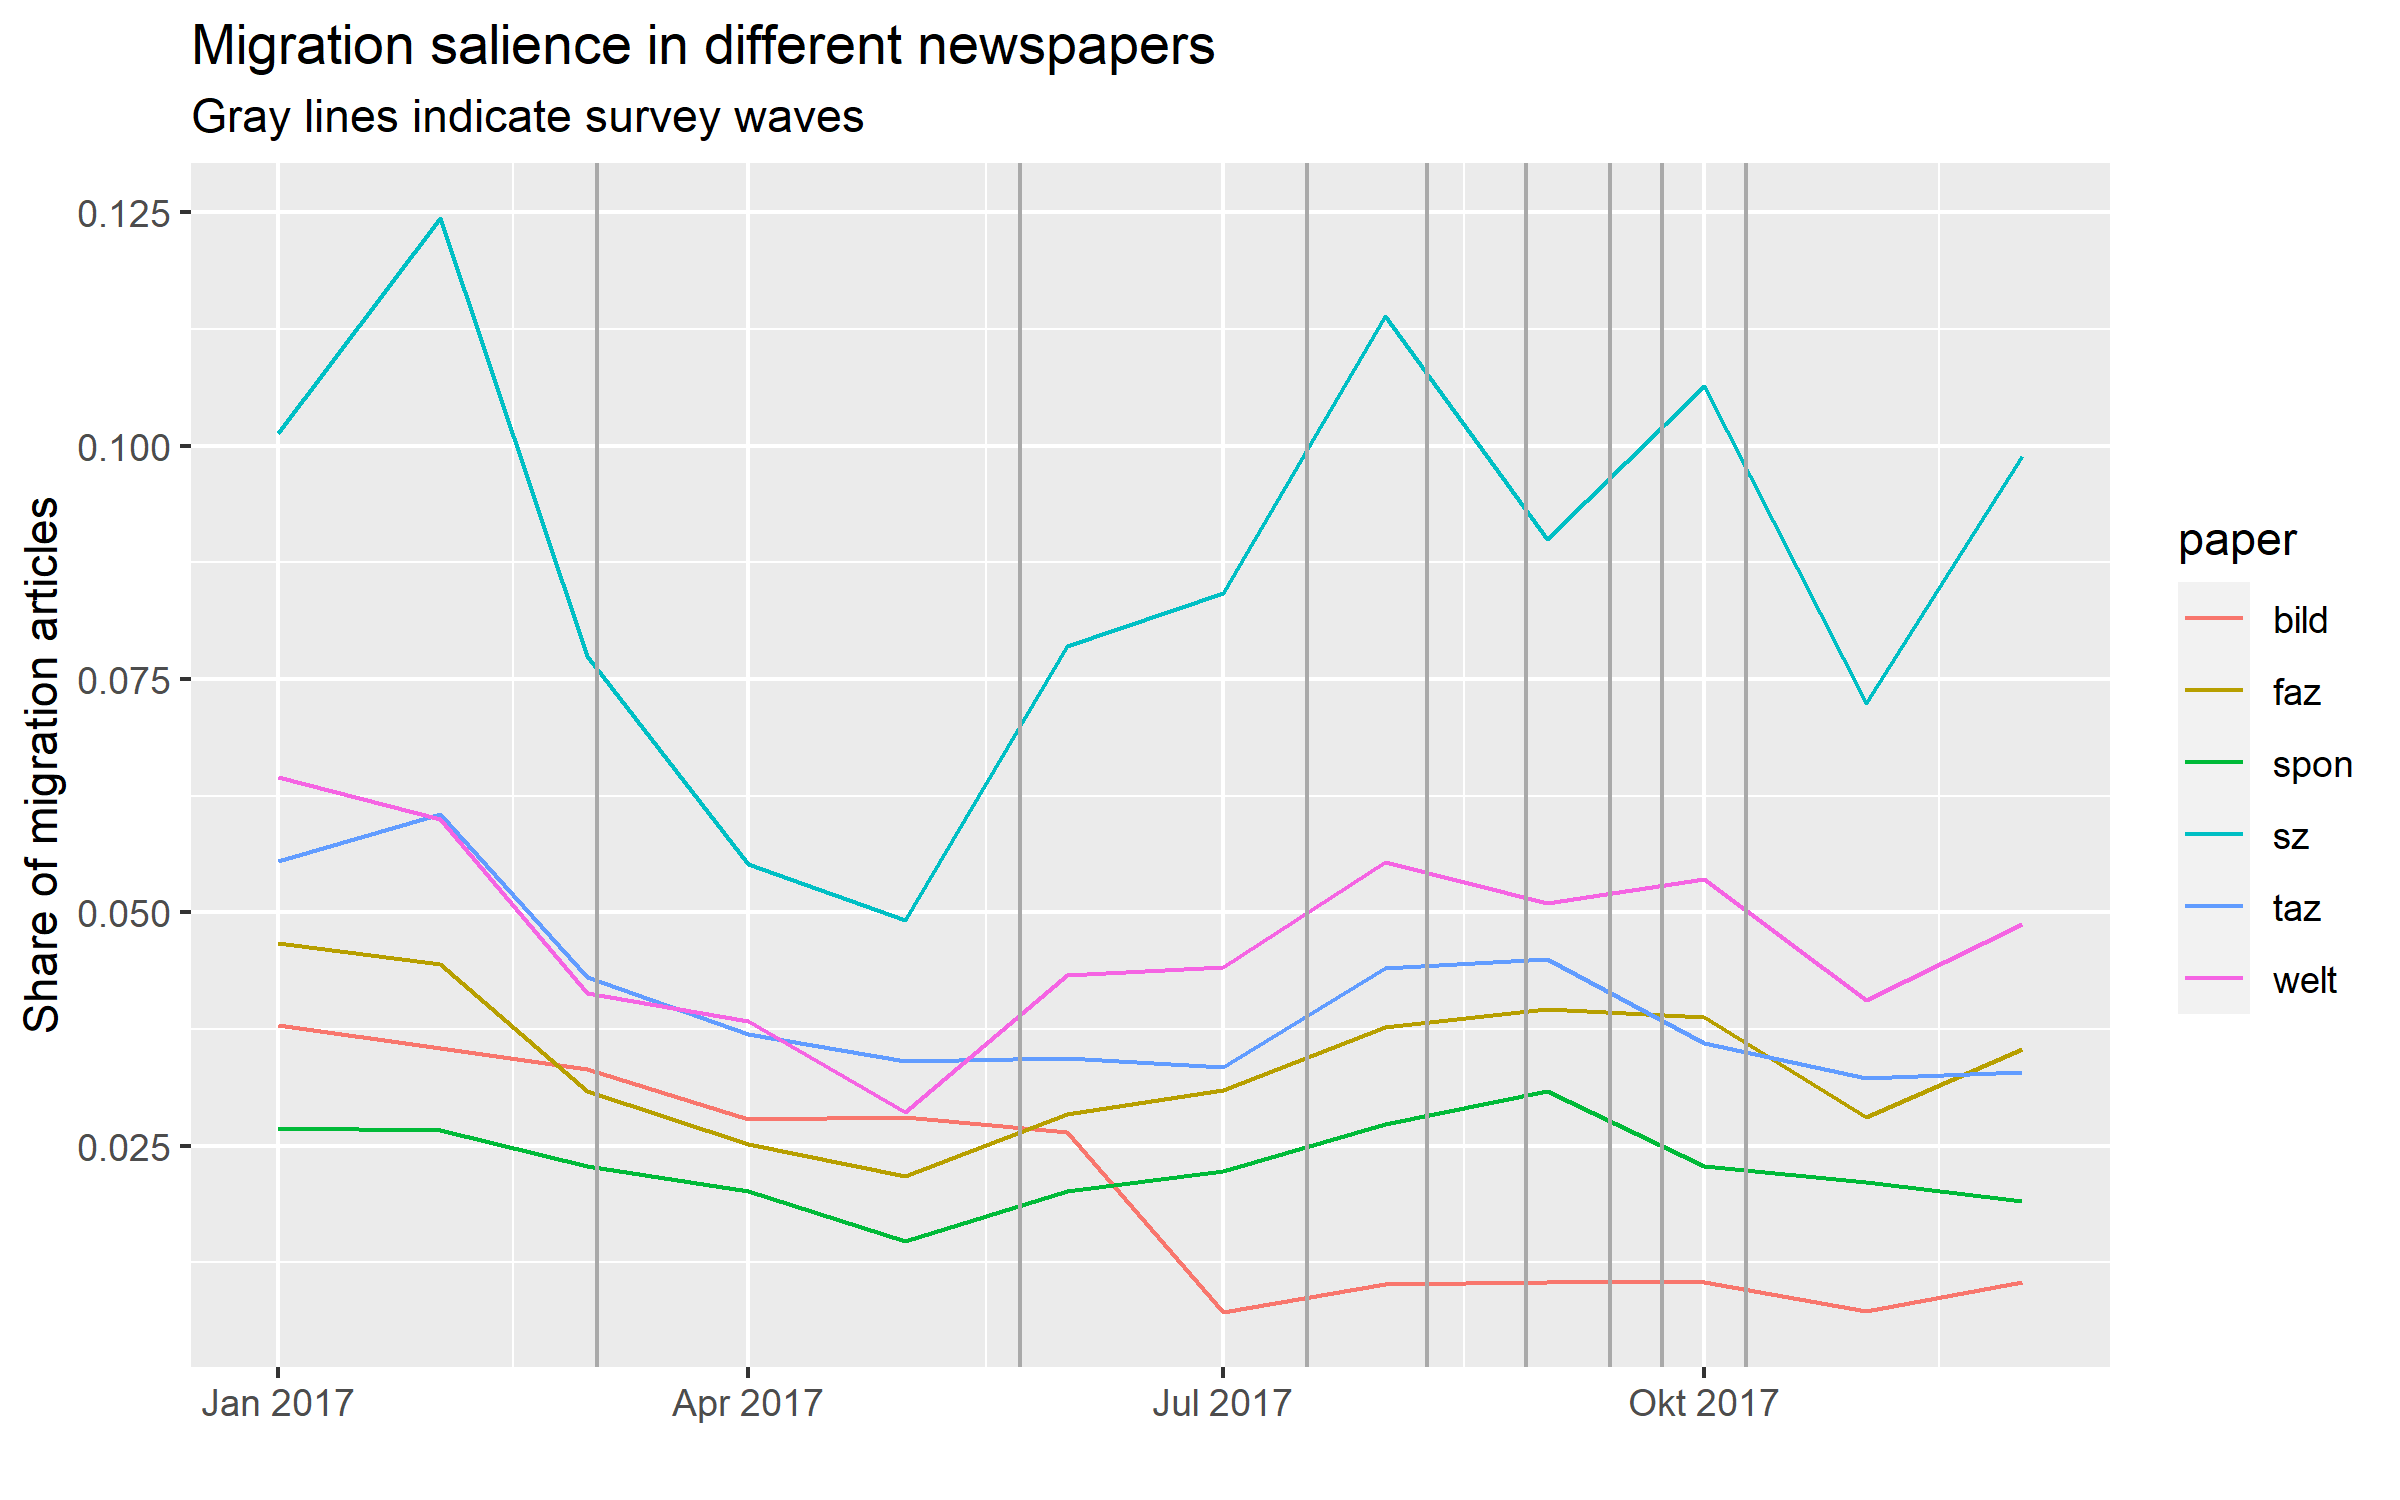
\includegraphics[width=\textwidth]{paper/vis/salience_papers_focus.png}
    \caption{Share of migration articles out of all articles across time for different newspapers.}
    \label{fig:salience}
\end{figure}


\subsubsection{Measuring news frames}

\begin{figure}[!ht]
    \centering
    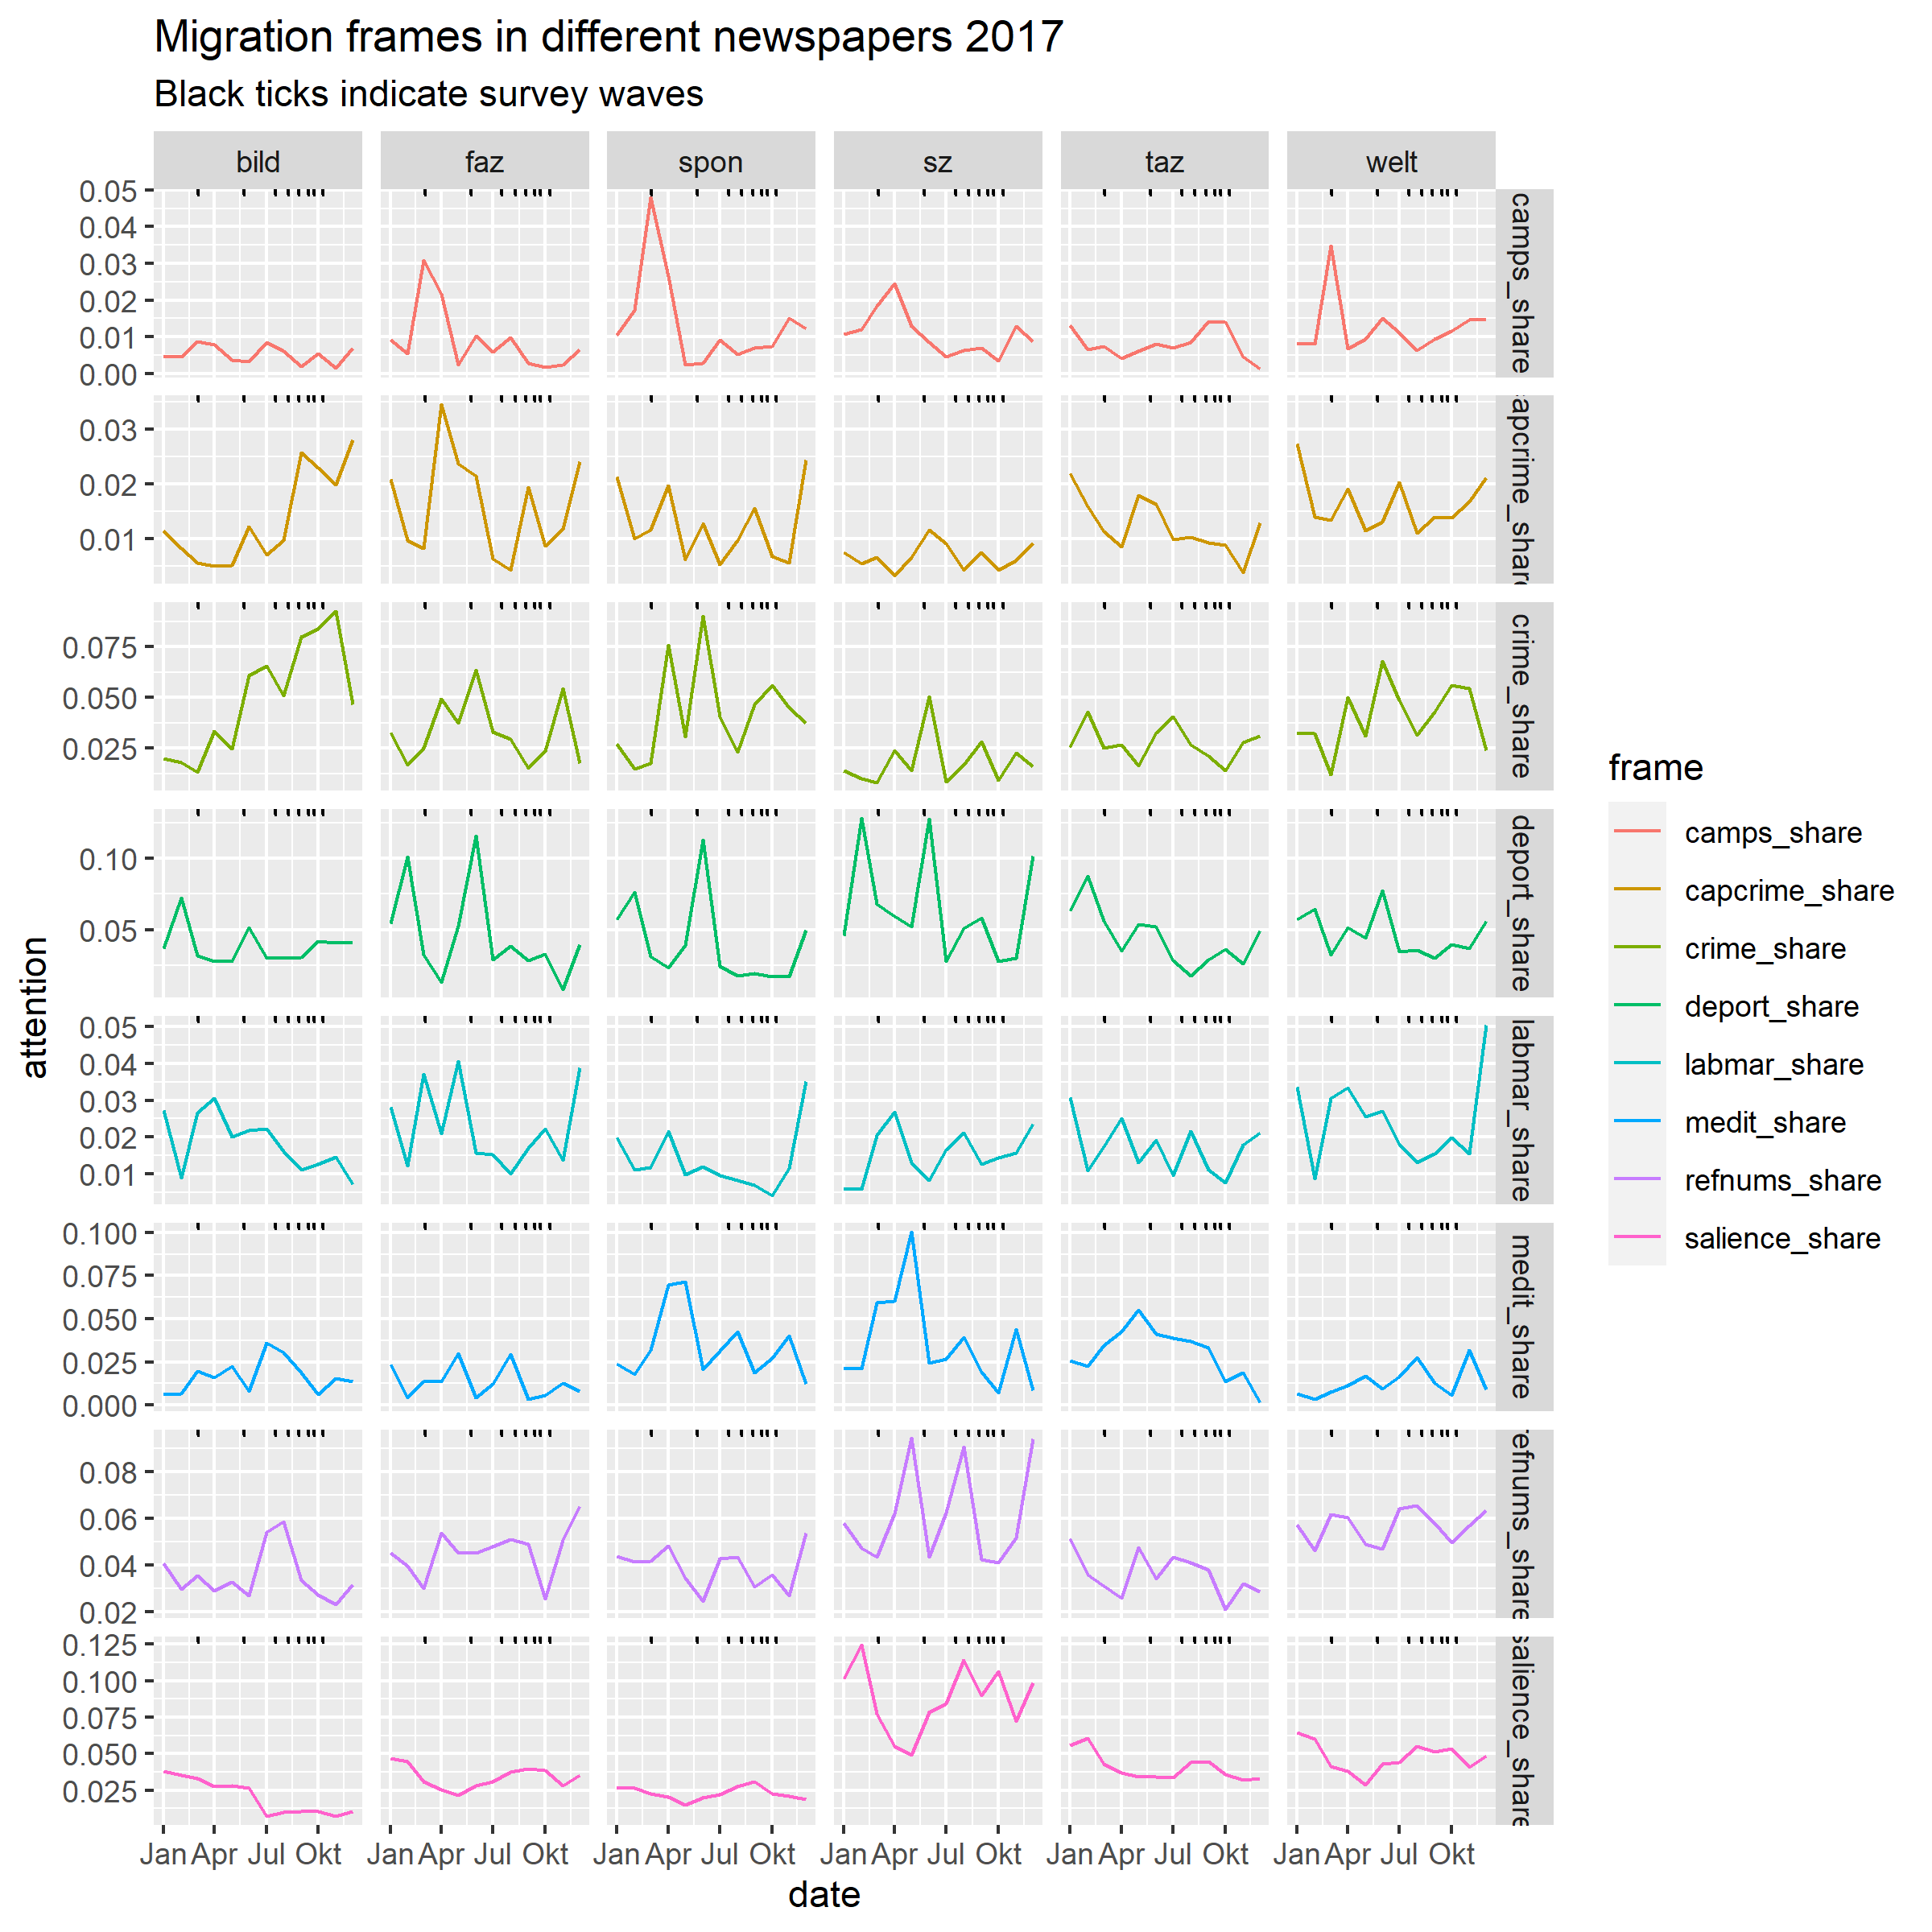
\includegraphics[width=\textwidth]{paper/vis/frames_papers_focus.png}
    \caption{Prevalence of different migration frames across newspapers. Gray vertical lines indicate survey field dates.}
    \label{fig:frames}
\end{figure}

\begin{itemize}
    \item Collected around 2.5 million newspaper articles from six major newspapers
    \item Extracted and annotated a stratified sample of articles using a migration dictionary
    \item Trained a migration classifier (BERT transformer) based on these annotations
    \item estimated migration frames using STM on migration articles only (N = 90,000): 
    \item retained most common and relevant frames that allow to form clear hypotheses about attitude formation:
    \begin{itemize}
        \item Internment camps, 
        \item capital crime (sexual assault/rape/murder) committed by refugees, 
        \item general petty crime by refugees and issues in refugee living quarters in Germany,
        \item deportations,
        \item labour market needs for and integration of refugees
        \item drownings in the mediterranean
        \item refugee numbers
    \end{itemize}
\end{itemize}



\subsection{Study design}

\subsubsection{Can framing effects among newspaper readers be observed?}

To get a glimpse of whether opinion shifts might be influenced by news consumption, I estimate difference-in-differences models (DiDs) for all available combinations of news outlets (incl. TV news), issues, and survey waves. The main term of interest is the interaction of a binary indicator of readership of a certain outlet with a binary indicator which equals 1 for the current wave and 0 for the preceding wave. That means I measure the shift in opinions of the readership of a certain outlet, controlling for the changes taking place among consumers of other news.

\subsubsection{Can these opinion shifts be explained by changing media frames?}

\begin{itemize}
    \item look at migration, maybe a second issue: how strongly do DiD's correlate with changing frame prevalence/DiD of frame attention?
    \item look at how FE model DiD's change when controlling for newspaper attention/DiD
    \item add right-wing slant as second dependent using AfD-classifier
\end{itemize}

\section{Results}

\subsection{DiD-assumption: Parallel trends}

% refer to graph on mig issue
The parallel trends assumption is met, as can be seen in figure \ref{fig:issues}. A plot of all other issues showing similar co-variation will be added to the appendix at a later point in time.
    
% also think about excludability: how can you ensure that these shifts are a result of media framing (this might be answered in number two)

\subsection{Distribution of DiD-effect significance}

The upper panel of figure \ref{fig:p_values} shows the distribution of p-values for the DiD-term from 1,056 fixed-effect models with GLES Panel data. The distribution shows a considerable deviation from the expected uniform distribution (visible in the lower panel) were there no explaining variation in the DiD-term beyond the uniform effects of wave and paper readership. This means, more often than random, the opinions of consumers of certain news deviate from the opinions of other citizens.

% show distribution of p-values vs theoretical distribution -> looks like there is systematic deviation
\begin{figure}[!ht]
    \centering
    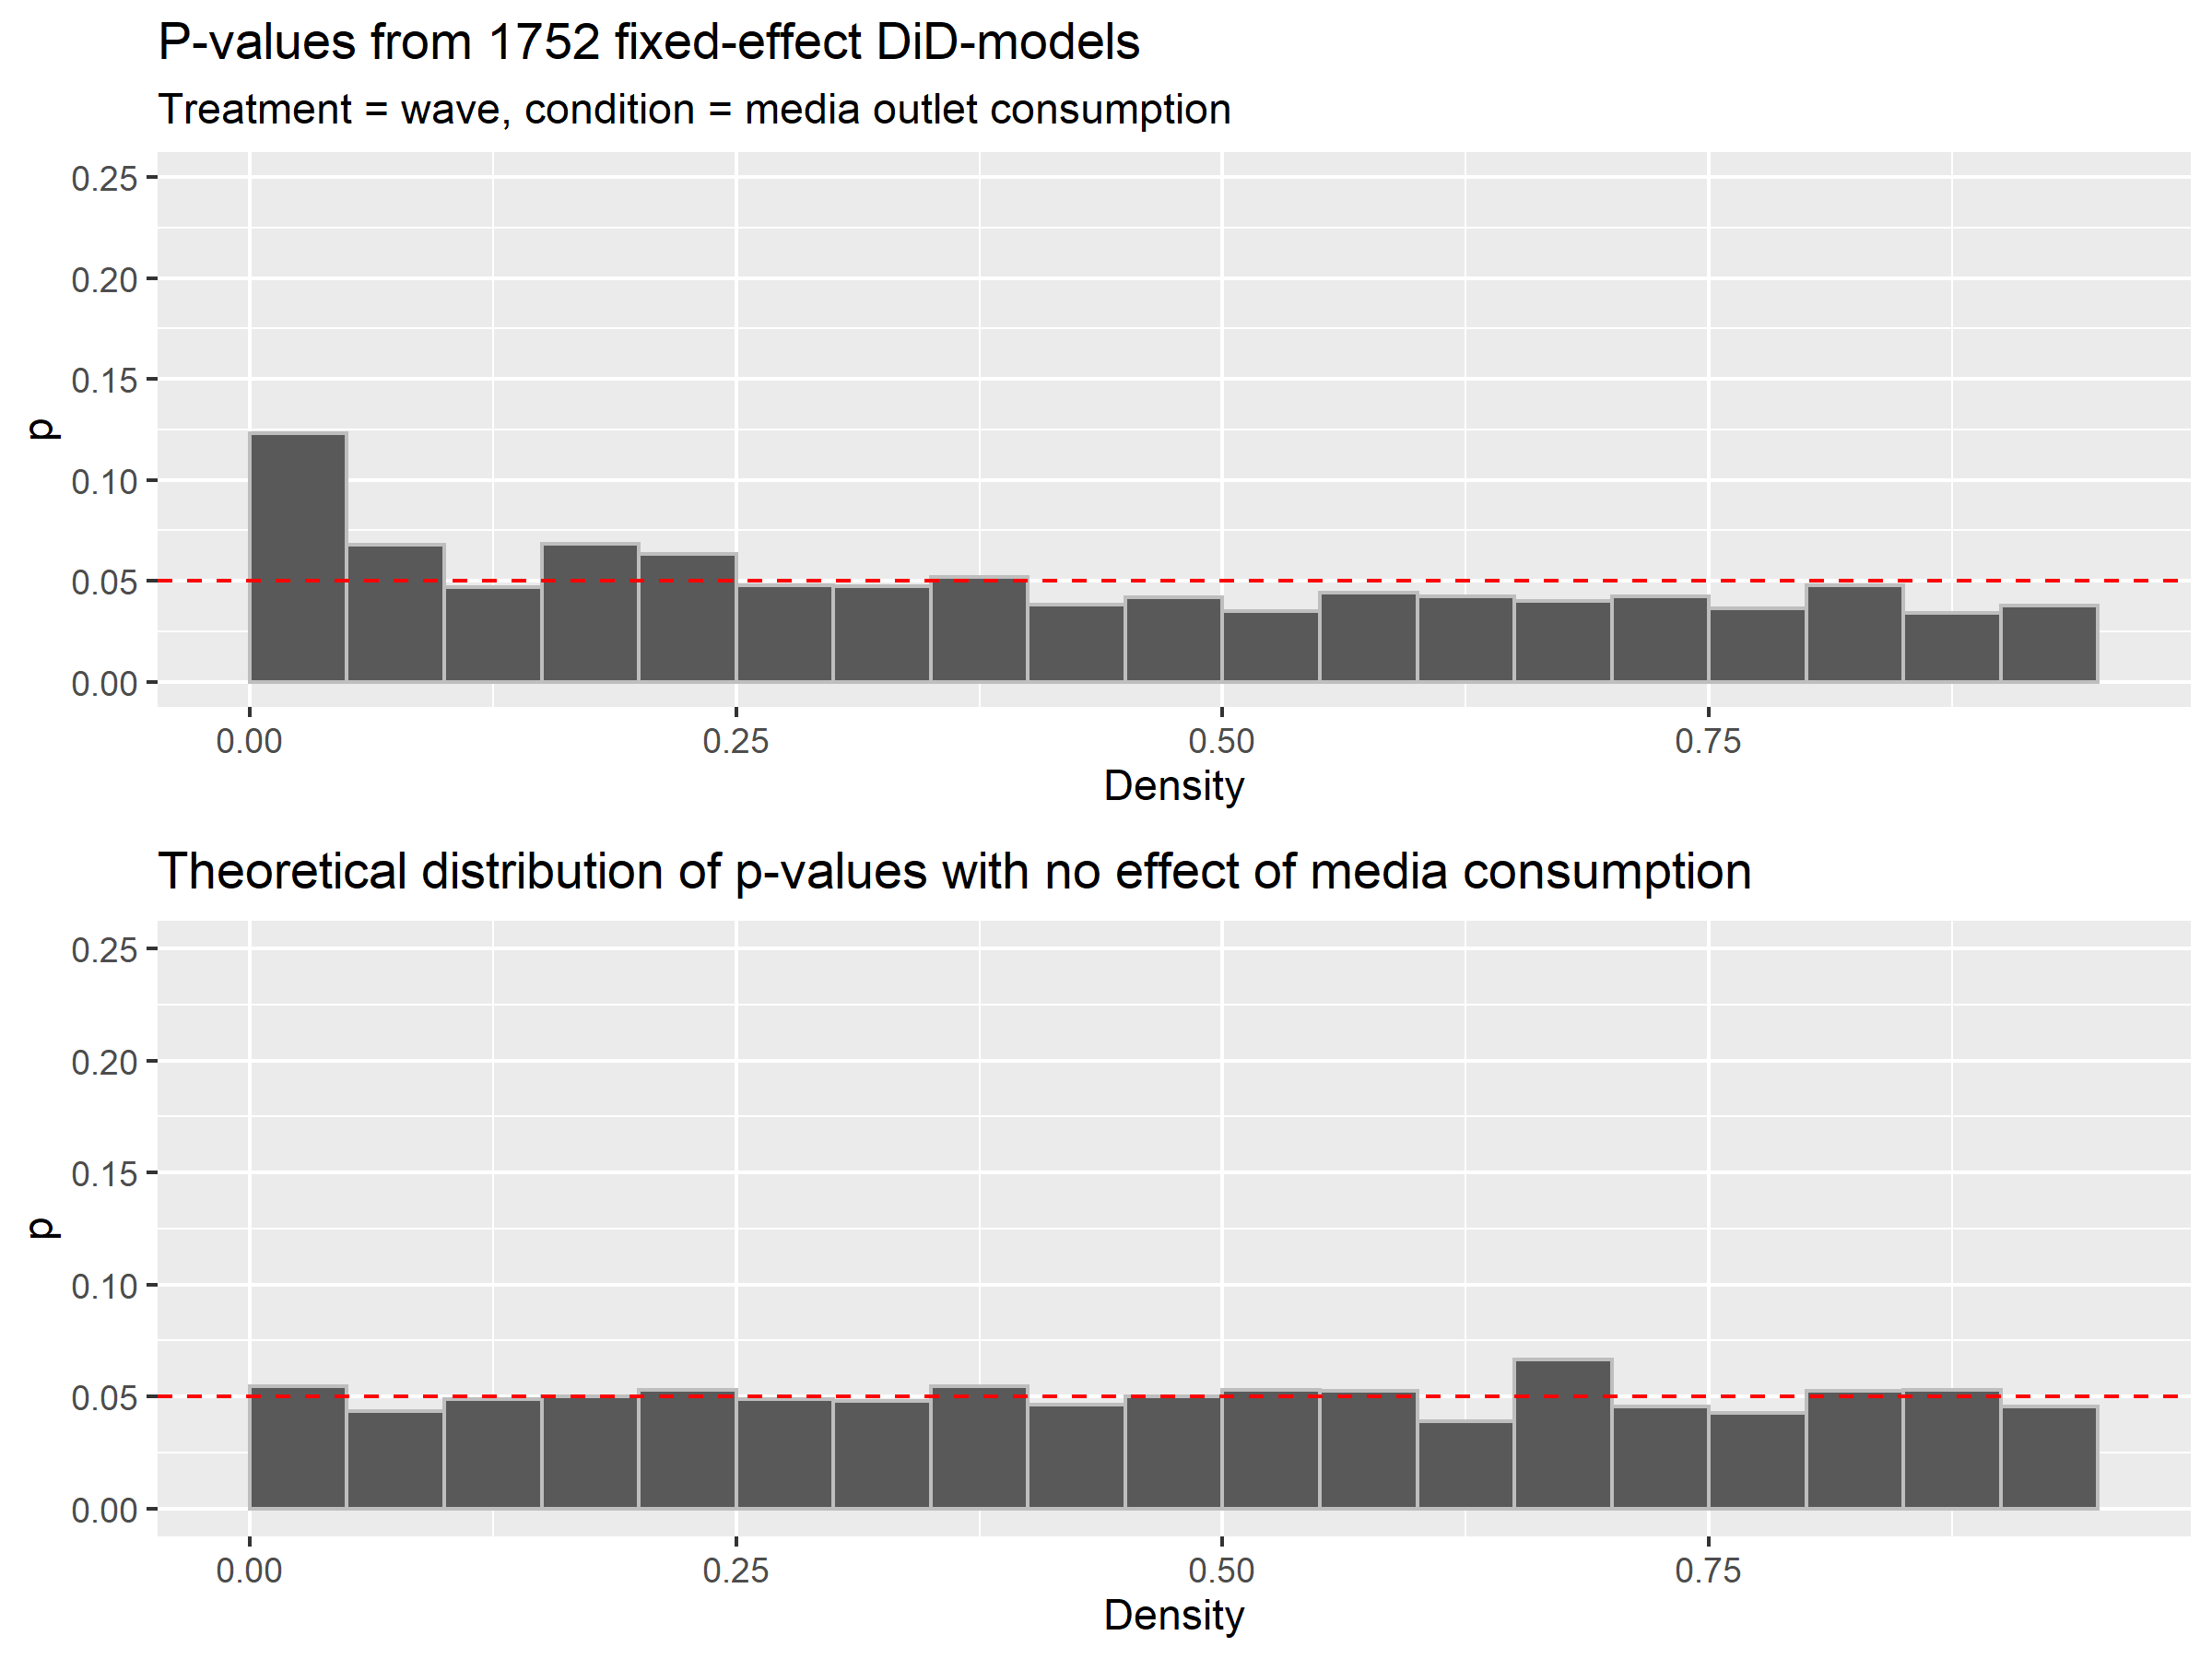
\includegraphics[width=\textwidth]{paper/vis/DiD_model_ps.png}
    \caption{Empirical and theoretical p-values of 1,363 DiD-models.}
    \label{fig:p_values}
\end{figure}



\subsection{Correlation of DiD with frame prevalence}
% show correlation of DiD with prevalence of media frames (STM)
\begin{figure}[!ht]
    \centering
    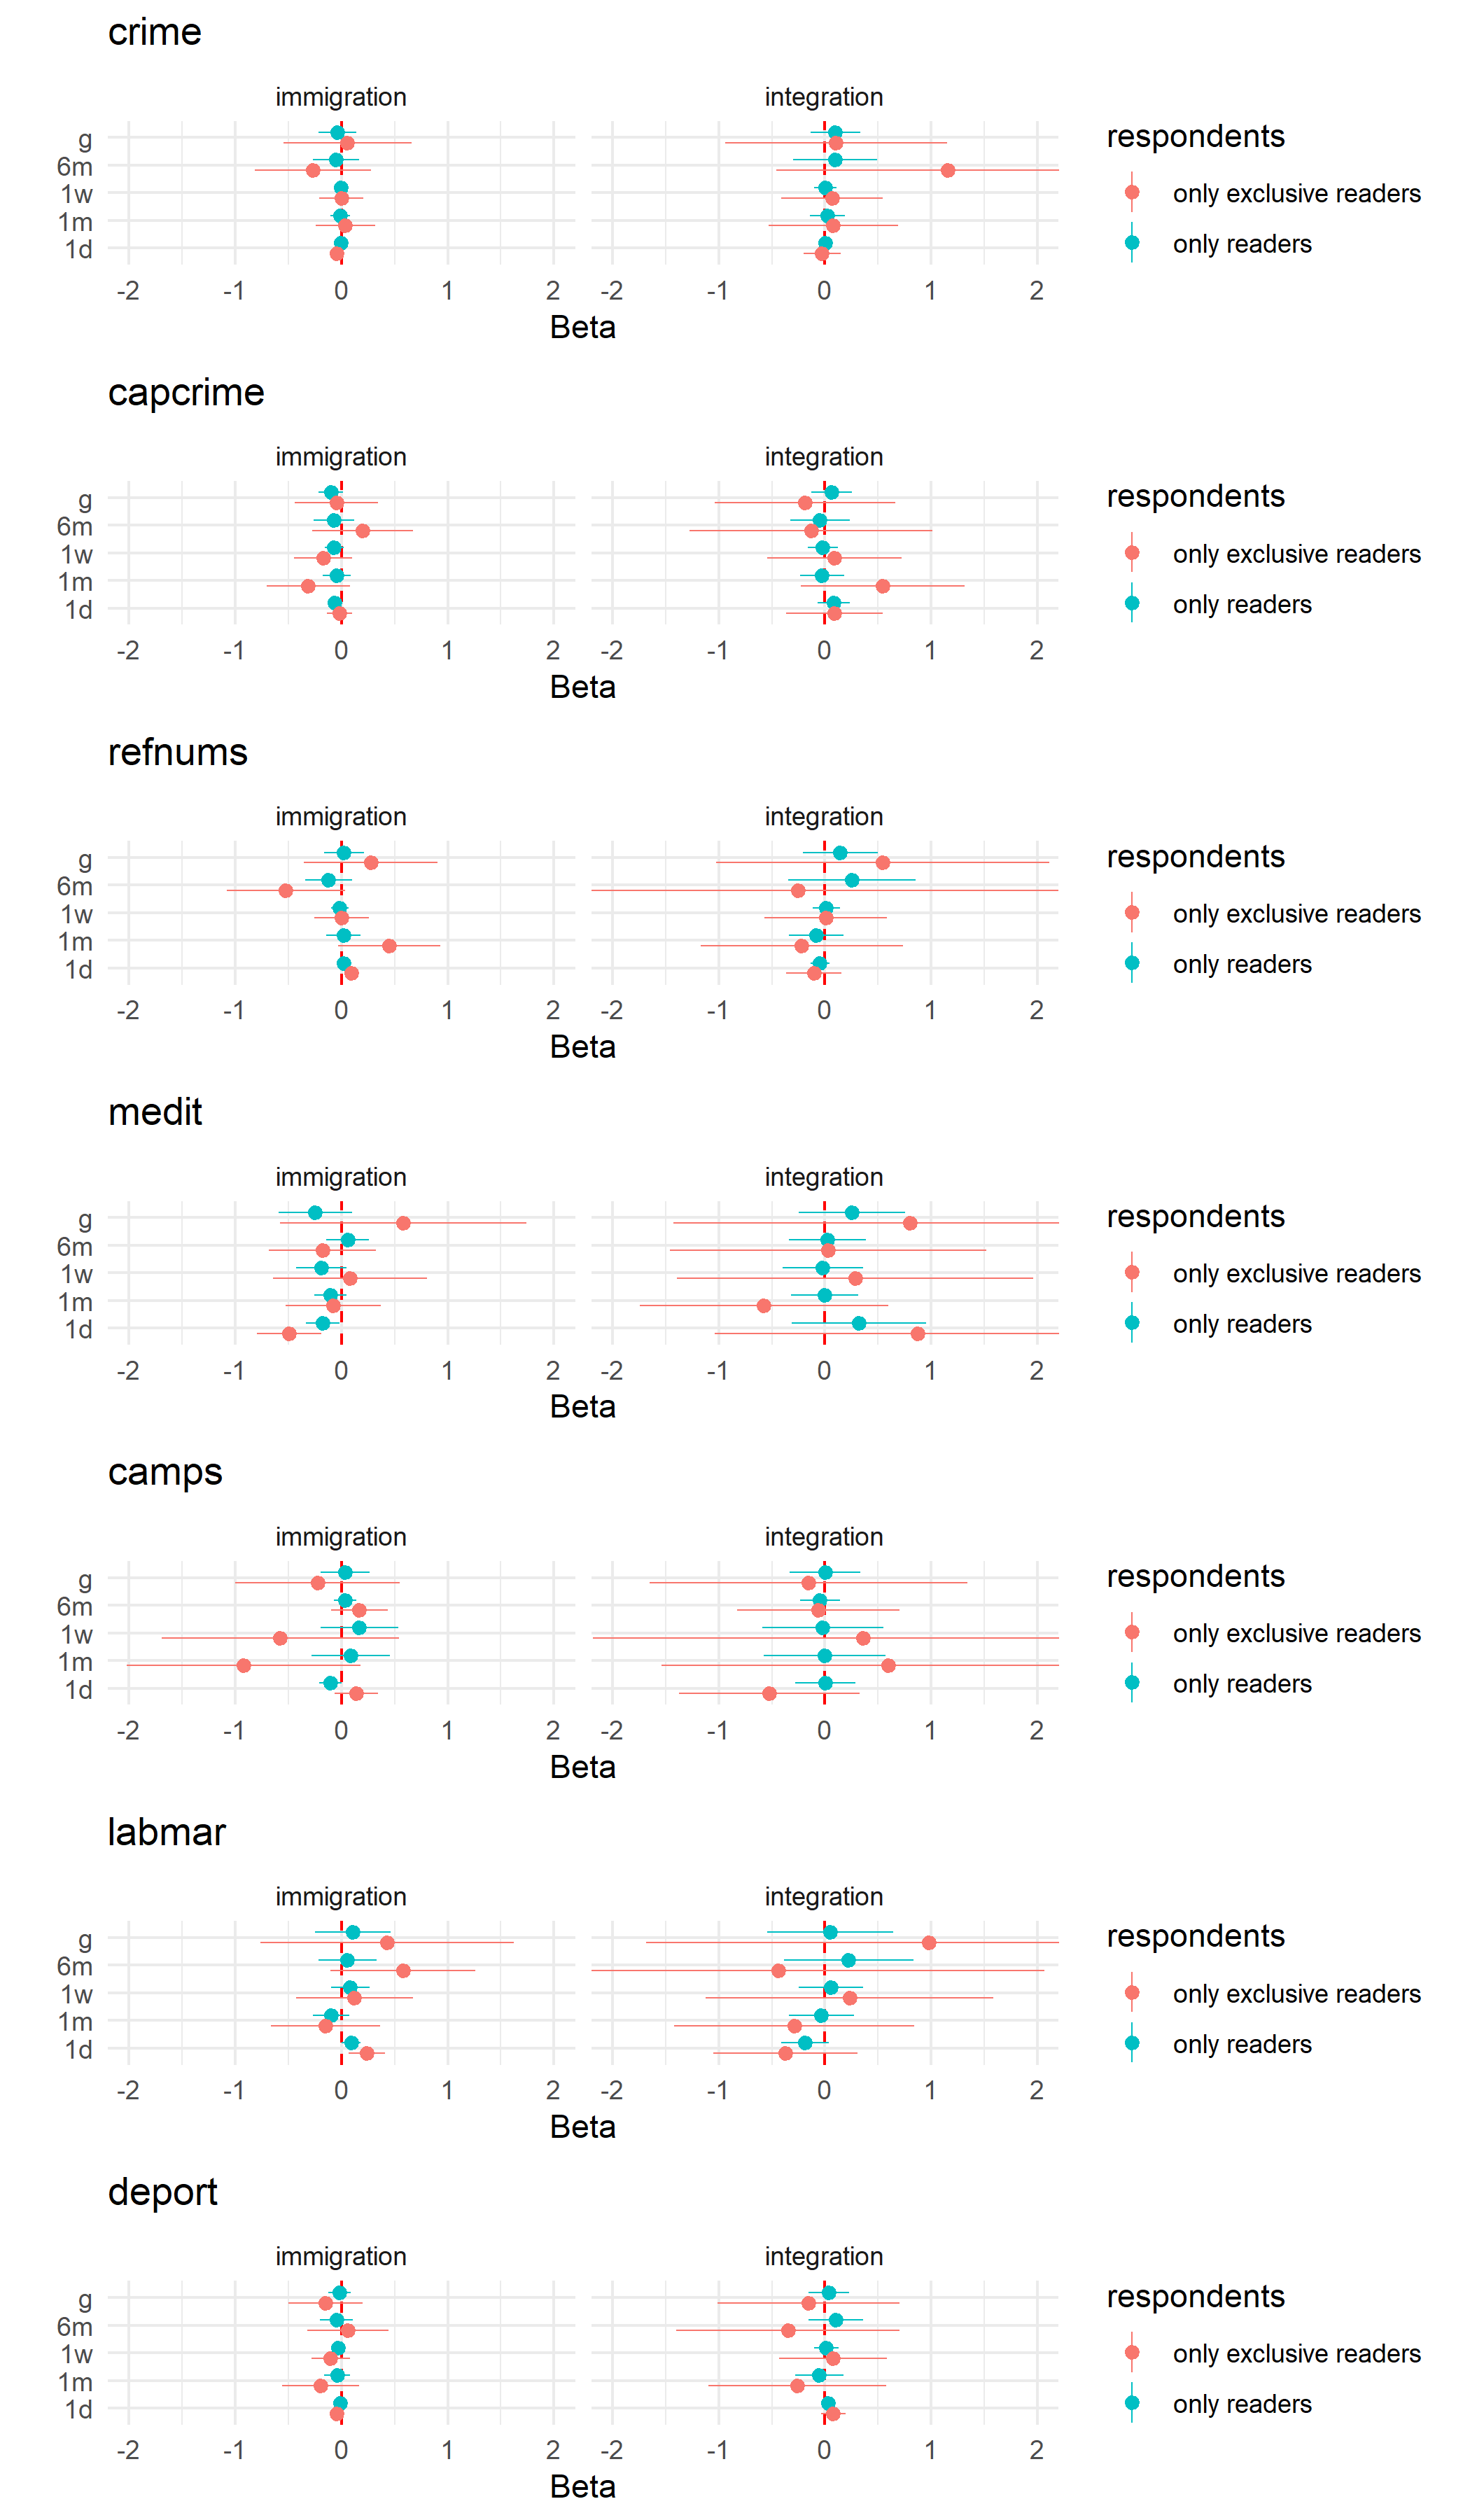
\includegraphics[width=\textwidth]{paper/vis/effectplot_frames.png}
    \caption{Correlation of opinion shifts (DiDs) with media attention or shifts in attention (DiD's) for different specifications.}
    \label{fig:did_corr}
\end{figure}

Figure \ref{fig:did_corr} shows the core analysis to estimate the effect of media attention on reader opinion. Each dot in this graph represents the t-value of a model explaining aggregate opinion shifts (DiDs, blue dots) with aggregate media attention or shifts in attention (DiDs) for a specific frame and a specific model specification. These aggregate parameters come from models explaining immigration opinion/media attention with news outlet-wave interactions, as in the models providing the p-values for figure \ref{fig:p_values}. If opinion shifts among newpapers' readers - relative to other readers - can be explained by shifts in newspapers' issue framing, these two variables should be highly correlated. The displayed estimates are hence obtained by regressing the resulting DiD-estimates for issue attitudes on the DiD-estimates for media attention.

For example, the left graph in the top panel row shows the effect of media attention on immigration attitudes for two different independent variables (DiD \textit{coef}ficients estimating the increase in news coverage in the consumed outlet relative to all others, and the general \textit{attention} in the preceding period) and four different time lags (see horizontal lines in descending order: 1 week, 1 month, 6 months, and the full period until last survey wave [g]). Note that immigration and integration are inversely coded. Higher values indicate more restrictive attitudes on immigration, but more liberal attitudes on integration. +/- signs corresponding to the frames (visible on the right-hand side) indicate the hypothesized effect of the frame on integration.


% show for one specific case that shift in media frame corresponded to 
\begin{table}[!htbp] \centering 
  \caption{Individual-level Model} 
  \label{} 
\begin{tabular}{@{\extracolsep{5pt}}lcc} 
\\[-1.8ex]\hline 
\hline \\[-1.8ex] 
 & \multicolumn{2}{c}{\textit{Dependent variable:}} \\ 
\cline{2-3} 
\\[-1.8ex] & Immigration attitude & Integration attitude \\ 
\\[-1.8ex] & (1) & (2)\\ 
\hline \\[-1.8ex] 
 Lagged DV & 0.793$^{***}$ & 0.664$^{***}$ \\ 
  &  & (0.004) \\ 
  & & \\ 
 Petty Crime & 0.0001 & 0.002 \\ 
  & (0.002) & (0.004) \\ 
  & & \\ 
 Capital Crime & 0.033$^{***}$ & $-$0.027$^{**}$ \\ 
  & (0.006) & (0.012) \\ 
  & & \\ 
 Refugee Numbers & $-$0.016$^{***}$ & $-$0.001 \\ 
  & (0.002) & (0.004) \\ 
  & & \\ 
 Refugee Camps & 0.025$^{***}$ & $-$0.004 \\ 
  & (0.004) & (0.012) \\ 
  & & \\ 
 Mediterranean S\&R & 0.035$^{***}$ & $-$0.005 \\ 
  & (0.002) & (0.005) \\ 
  & & \\ 
 Labour Market & 0.015$^{***}$ & 0.009 \\ 
  & (0.003) & (0.006) \\ 
  & & \\ 
 Deportation & $-$0.002$^{***}$ & 0.002$^{**}$ \\ 
  & (0.001) & (0.001) \\ 
  & & \\ 
 Constant & 0.045$^{***}$ & $-$0.288$^{***}$ \\ 
  & (0.015) & (0.036) \\ 
  & & \\ 
\hline \\[-1.8ex] 
Observations & 88,026 & 36,180 \\ 
R$^{2}$ & 0.617 & 0.421 \\ 
Adjusted R$^{2}$ & 0.617 & 0.421 \\ 
Residual Std. Error & 1.095 (df = 88017) & 1.095 (df = 36171) \\ 
F Statistic & 17,740.240$^{***}$ (df = 8; 88017) & 3,286.942$^{***}$ (df = 8; 36171) \\ 
\hline 
\hline \\[-1.8ex] 
\textit{Note:}  & \multicolumn{2}{r}{$^{*}$p$<$0.1; $^{**}$p$<$0.05; $^{***}$p$<$0.01} \\ 
\end{tabular} 
\end{table}


\section{Discussion}
\begin{itemize}
    \item 
    \item people could a) not react, b) stop reading their newspaper, c) change their opinion
\end{itemize}

\section{Appendix}

\subsection{Descriptives on issue importance across time and newspaper consumption}\label{app:importance}

[add description and plot issue importance]

\end{document}